\documentclass[11pt]{article}

% Handle Spanish seamlessly!
\usepackage[utf8]{inputenc}
\usepackage[spanish, es-tabla]{babel}

% Change the language for the captions and default names
\renewcommand{\figurename}{Figura}

% Needed for the multline environment
\usepackage{amsmath}

% Images
\usepackage{graphicx}
\graphicspath{{Img/}}

\usepackage{geometry}
\geometry{
    a4paper,
    left = 20mm,
    right = 20mm,
    top = 15mm,
    bottom = 15mm
}

% Links please!
\usepackage{hyperref}

% Format the links
\hypersetup{
    pdfborder = {0 0 0},    % Remove the ugly border
    colorlinks = true,      % Let there be color
    citecolor = black,      % Make citations appear normal (i.e black)
    linkcolor = black,      % The same for links (i.e table of contents)
    urlcolor = cyan         % Color the web links. (cyan is fancy for blueish...)
}

\title{Conformando trafico}
\author{Pablo Collado Soto \\ \\ \textit{Ingeniería de Tráfico}}
\date{}

\begin{document}
    \maketitle

    \section{Introducción}
        En esta práctica comenzaremos por estudiar el funcionamiento de un clasificador \textit{WFQ} de manera práctica a través de la simulación de un escenario análogo al de la práctica anterior. Más tarde analizaremos un clasificador \textit{WFQ} de manera teórica para terminar con el estudio de un conformador de tráfico según un cubo con goteo así como una función policía basada en el mismo algoritmo.

    \section{Estudiando un clasificador \textit{WFQ} (2.1.1)}
        Antes de nada definiremos los flujos de nuestro escenario en la tabla \ref{tab:wfqFlows}. Debemos tener en cuenta que la velocidad de la interfaz de salida de los flujos de datos es $V_l = 10\ Mbps$ para toda la prueba. La configuración del router para este escenario se puede encontrar \href{https://github.com/UAH-s-Telematics-Engineering-Tasks/traff_eng/blob/master/P2/Router_confs/originalWFQ.cfg}{aquí}.

        \begin{table}
            \centering
            \begin{tabular}{|c|c|c|c|c|c|c|}
                \hline
                & \texttt{Puerto} & \texttt{Comienzo [s]} & \texttt{Fin [s]} & \texttt{Tasa [Mbps]} & \texttt{Paquetes por segundo} & \texttt{SDU de UDP [B]}\\
                \hline
                1 & 51151 & 0 & 20 & 8 & 800 & 1250\\
                \hline
                2 & 51152 & 5 & 20 & 1,5 & 150 & 1250\\
                \hline
                3 & 51153 & 10 & 20 & 4 & 400 & 1250\\
                \hline
                4 & 51154 & 15 & 20 & 2,4 & 240 & 1250\\
                \hline
                5 & 51155 & 15 & 20 & 1,6 & 160 & 1250\\
                \hline
            \end{tabular}
            \caption{Configuración de los flujos para estudiar \textit{WFQ}.}
            \label{tab:wfqFlows}
        \end{table}

        \subsection{Comentando las figuras}
            Observando la tasa de cada flujo en la figura \ref{fig:wfqOriginalR} vemos que, en efecto, se garantiza que el \texttt{flujo 2} mantiene la tasa durante la prueba. Tengamos en cuenta que el flujo tiene una tasa de $1,5\ Mbps$ mientras que a este flujo se le otorgan $5\ Mbps$ al tener un peso del $50\%$ de la velocidad de la interfaz. Concluimos pues que las tasas son congruentes con lo esperado.\\

            Analizando la latencia que aparece en la figura \ref{fig:wfqOriginalLat} veremos que a medida que se añaden más flujos a la prueba se empiezan a saturar los buffers asociados a cada flujo \textbf{exceptuando} el \texttt{flujo 2} ya que éste nunca superará la tasa que tiene asociada. En los instantes iniciales de la prueba solo contamos con los flujos \texttt{1 y 2} cuyo total agregado es de $9,5\ Mbps < V_l = 10\ Mbps$ con lo que se puede acomodar todo el tráfico al repartirse la capacidad no asociada a otros flujos con lo que la latencia es prácticamente $0\ s$. Cuando los siguientes flujos entran en acción su capacidad asociada no puede ser empleada para el primer flujo con lo que la latencia comienza a dispararse. Llegará un momento en el que todos los flujos excepto el \texttt{2} saturen su cola asociada que ocurre cuando llegan a una línea horizontal. Esta latencia máxima de cola es $85\ ms$ y $400\ ms$ para los flujos \texttt{1} y \texttt{3, 4 y 5}, respectivamente.

            \begin{figure}
                \centering
                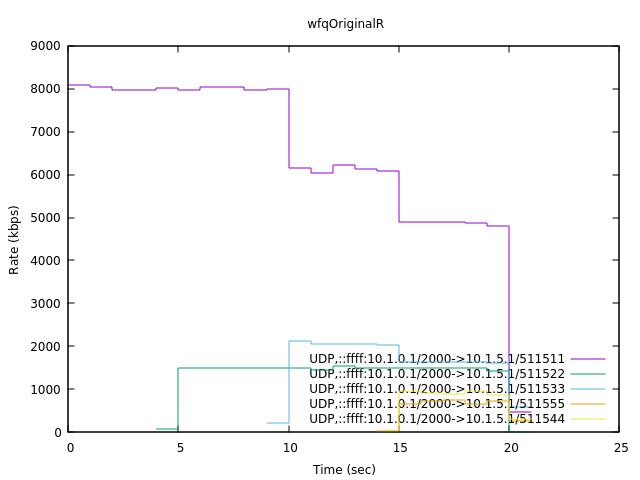
\includegraphics[width=0.6\linewidth]{wfqOriginalR.png}
                \caption{Tasa de cada flujo.}
                \label{fig:wfqOriginalR}
            \end{figure}

            \begin{figure}
                \centering
                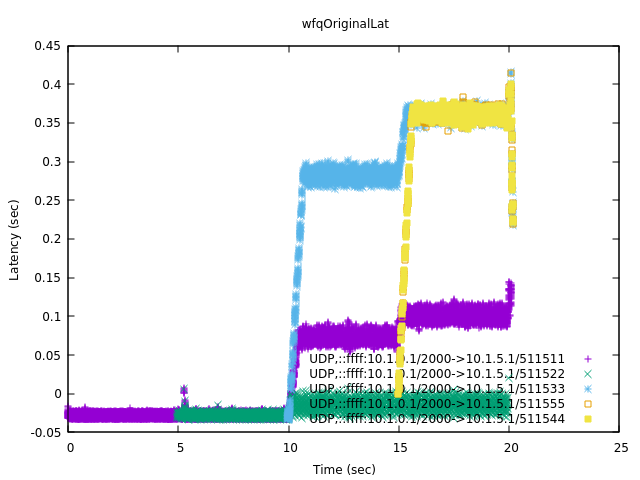
\includegraphics[width=0.6\linewidth]{wfqOriginalLat.png}
                \caption{Latencia de cada flujo.}
                \label{fig:wfqOriginalLat}
            \end{figure}

    \section{Garantizando una latencia mínima con \textit{WFQ} (2.1.2)}
        Empleando los mismos flujos que en el apartado anterior vamos a priorizar uno de los flujos de manera que solo se saquen paquetes de otras colas si y solo si esta cola prioritaria está vacía. Como esto podría provocar inanición, la implementación práctica descartará el tráfico prioritario en exceso (según el porcentaje configurado) a no ser que las demás colas estén vacías. Ésto se traducirá en que se mantendrá una latencia acotada pero se incrementarán las pérdidas del flujo prioritario a medida que se añadan más flujos a la prueba. La configuración del router para este caso se puede encontrar \href{https://github.com/UAH-s-Telematics-Engineering-Tasks/traff_eng/blob/master/P2/Router_confs/prioWFQ.cfg}{aquí}, siendo la única diferencia con la anterior la línea \texttt{58}.

        \subsection{Comentando las figuras}
            Tal y como comentábamos al explicar la implementación de las prioridades observamos cómo la tasa del flujo prioritario (el \texttt{1}) empezará en los $8\ Mbps$ iniciales hasta que se incorporan más flujos. Al hacerlo, la tasa se irá reduciendo hasta que en los últimos $5\ segundos$ se aproxima a $1\ Mbps$, el $10\%$ de la velocidad del interfaz que configuramos. Todo esto se observa en la figura \ref{fig:wfqPrioR}.\\

            Si observamos la latencia en la figura \ref{fig:wfqPrioLat} nos daremos cuenta de que, como antes, la latencia del flujo \texttt{2} se mantiene constante al tener asignado suficiente ancho de banda y que \textbf{además} la latencia del flujo \texttt{1} también está acotada al ser el flujo prioritario. Las demás tasas se comportan como comentábamos antes.\\

            Si acabamos por observar las pérdidas en la figura \ref{fig:wfqPrioLoss} nos daremos cuenta de que las pérdidas de todos los flujos excepto el \texttt{2} experimentarán pérdidas hacia el final de la prueba. Si nos centramos en el flujo \texttt{1}, el prioritario, veremos que estas pérdidas comienzan a dispararse en cuanto el tercer flujo entra en acción y debemos empezar a descartar paquetes. Es interesante ver que el aumento de las pérdidas del flujo \texttt{1} se produce en el mismo instante en el que su tasa se disminuye.

            \begin{figure}
                \centering
                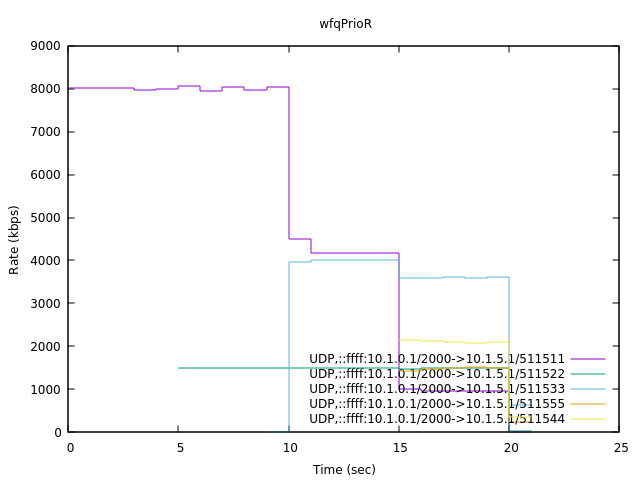
\includegraphics[width=0.6\linewidth]{wfqPrioR.png}
                \caption{Tasa de cada flujo.}
                \label{fig:wfqPrioR}
            \end{figure}

            \begin{figure}
                \centering
                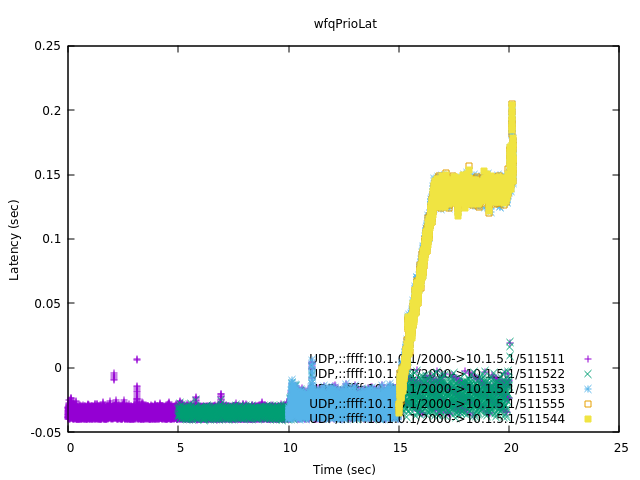
\includegraphics[width=0.6\linewidth]{wfqPrioLat.png}
                \caption{Latencia de cada flujo.}
                \label{fig:wfqPrioLat}
            \end{figure}

            \begin{figure}
                \centering
                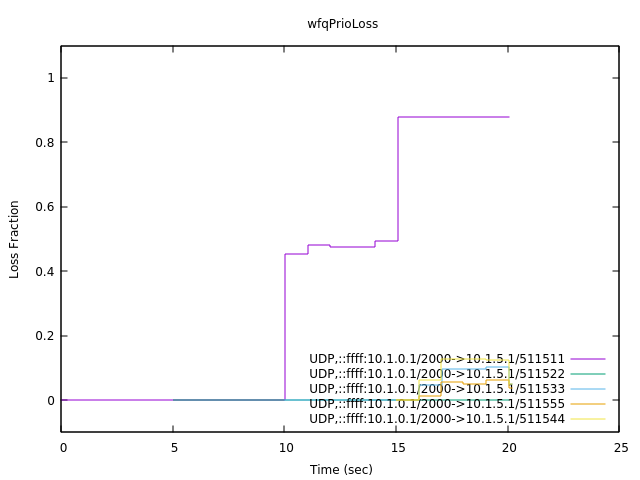
\includegraphics[width=0.6\linewidth]{wfqPrioLoss.png}
                \caption{Pérdidas de cada flujo.}
                \label{fig:wfqPrioLoss}
            \end{figure}

\end{document}
